\documentclass[12pt,halfline,a4paper]{ouparticle}
% *
%
% ^.
\usepackage{amsmath,amssymb}
\usepackage{natbib}
\usepackage{graphicx,rotating}
\usepackage{dsfont}

\newcommand{\Est}[1]{\hat{#1}}

\newcommand{\beginsupplement}{%
        \setcounter{table}{0}
        \renewcommand{\thetable}{S\arabic{table}}%
        \setcounter{figure}{0}
        \renewcommand{\thefigure}{S\arabic{figure}}%
     }
\newcommand{\stopsupplement}{%
        \setcounter{table}{0}
        \renewcommand{\thetable}{\arabic{table}}%
        \setcounter{figure}{0}
        \renewcommand{\thefigure}{\arabic{figure}}%
     }

% method names

\newcommand{\stdpopsim}{\texttt{stdpopsim} }
\newcommand{\dadi}{\texttt{dadi} }
\newcommand{\MSMC}{\texttt{MSMC} }
\newcommand{\smcpp}{\texttt{smcpp} }
\newcommand{\stairwayplot}{\texttt{stairwayplot} }
\newcommand{\fastsimcoal}{\texttt{fastsimcoal} }

\newcommand{\adk}[1]{\textcolor{red}{ADK: #1}}

\usepackage[colorinlistoftodos]{todonotes}

\begin{document}

\title{\stdpopsim: a community-supported toolkit for population genetic simulation}

\author{%
\name{The PopSim Consortium}
\address{}
\email{}}


\abstract{The explosion in population genomic data demands ever increasingly complex modes of analysis.
More and more these analyses depend on sophisticated, often computationally expensive simulation.
To date, computational genetics researchers have been often forced to re-implement such simulations
independently, leading to both wasted time in the duplication of effort and reductions in reproducibility.
Population genetics, as a field, specifically lacks rigorous standard benchmarks by which new tools for inference might
be measured. Here we describe a new resource, the PopSim library, that attempts to rectify this situation.
PopSim is a community-driven, open source project, aimed at revolutionizing the ease and reproducibility
of population genetic simulation for a catalog of published demographic models from both humans and non-model organisms.
PopSim assures correctness in our implementations through a mature quality control pipeline that is
community-based. Here we describe the PopSim resource as a step towards inviting an even broader
community of developers to participate and demonstrate some rather simple examples of how one
might use PopSim for comparison of methods of demographic inference.}

\date{\today}

\keywords{Population genetics, Simulation, Inference}

\maketitle


\section*{Introduction}
While population genetics has always used statistical methods to make inferences from data,
the degree of sophistication of the questions, models, data, and computational approaches
used have all increased over the past decade. Currently there exist myriad computational methods
that can infer the histories of populations, the distribution of fitness effects,
recombination rates, the extent of positive selection in genome sequence data
(\cite{li2011inference,schiffels2014inferring,terhorst2017robust,eyre2009estimating,kim2017inference,
chan2012genome,lin2013fast,Adrion662247,alachiotis2012omegaplus,degiorgio2016sweepfinder2,
kern2018diplos,sugden2018localization}).
While en masse these methods have increased our understanding of the
impacts of genetic and evolutionary processes, very little has been done to systematically
benchmark the quality of inferences gleaned from computational population genetics.
This is in large part because ``ground-truth'' in population genetics comes from simulation,
not from empirical observations, and as a field there has been no agreement as to what should
constitute community standards or best practices. The general modus operandi to date has been to
introduce methods which are validated by a set of bespoke simulations produced by individual
groups. Beyond a lack of efficiency from duplicated effort, such a situation leads
to decreases in reproducibility and transparency across the entire field.
Here we describe the PopSim consortium project, a community-driven catalog
of standardized simulations across a variety of common study organisms
that will empower the field and usher in the next era of genetics data analysis.

Benchmarking method performance population genetics is not straightforward.
Many population genetic inference methods often make different assumptions as
well as use different summaries of the genetic variation data, even when
attempting to address the same biological question. For example, there are
numerous methods to infer population size changes.
The \MSMC method (\cite{schiffels2014inferring}) allows for the
population to continuously change in size over time. Other popular methods, like
\dadi (\cite{gutenkunst2009inferring}), typically allow for a smaller number of size changes to occur at certain
points throughout the population's history. Further, the types of data that the
methods use also differs. While \MSMC uses one to four whole genome sequences and leverages the
spatial patterns of genetic variation along the sequence, \dadi  instead uses the
site frequency spectrum (SFS), which summarizes the frequencies of SNPs in the
sample, ignoring any information about the correlation structure (linkage
disequilibrium) among SNPs. Thus from the start these methods may not be
expected to perform equally well in all scenarios. \adk{I think we are focussed
a bit too much on benchmarking currently in the intro. Could be good to add more on efficiency
and reproducibility}

The degree to which modeling assumptions and using different summaries of the
data can affect the ultimate results has been challenging to assess. Yet, there
have been several clear examples of different methods yielding fundamentally
different conclusions. For example, \MSMC methods applied to human genomes have
suggested large ancient (>100 years ago) ancestral population sizes and
bottlenecks that have not been detected by SFS-based methods (see
\cite{beichman2017comparison}). These distinct models differ in how they fit various summaries of the
genetic variation data, suggesting that modeling choices can greatly affect the
performance of the inference. Further it is reasonable
to assume generally that specific methods will perform better than others under certain scenarios.
However, because these conditions are typically unknown, empirical researchers
lack principled guidelines for deciding which statistical method is best suited
for to accurately answer their particular question. The need for empirical
guidance will only increase as researchers continue to generate more genomic
variation data from non-model taxa and wish to make inferences regarding
demography and selection.

One way to benchmark different methods for statistical inference in population
genetics is to apply the methods to simulated datasets where the true model
parameters are known. Methods that perform well will accurately infer these
parameters and will also provide reasonable estimates of uncertainty of the
estimated parameters. Indeed simulations studies are a standard ingredient in
most papers proposing new methods in population genetics. However, these
simulation studies are often specifically devised to showcase the performance
of the novel method and may not adquately compare performance to competing
methods. Moreover researchers are generally forced to ``reinvent the wheel''
with respect to simulations, and are forced to reimplement previously
inferred scenarios independently. This can lead to errors being incorporated
during the implementation of the simulations. Lastly, the degree to
which different methods are compared can be quite variable.

One reason why simulation studies do not compare the performance of many methods
is that these simulation studies are challenging to carry out. There are several
practical impediments to carrying out the ideal benchmarking simulation studies.
First, while there are many published population genetic models available, their
parameters are often not easily accessible, often presented in supplemental
tables. Implementing these parameters into usable commands for simulations can
be a time-consuming and error prone process. Further, often papers present many
different models, and different authors may choose to select distinct models,
making comparison difficult. While improvements in simulation software and ever
faster computers have partially ameliorating this concern, generating the
simulated datasets stil can still be a time and computing resource bottleneck.

For these reasons, we have generated a standardized, community-driven resource
for simulation of published demographic models from a number of popular study systems.
This resource, which we call PopSim, significantly eases the development
burden of implementing realistic simulations for population genetic analysis.
Briefly, PopSim currently is comprised of a catalog of four organism genomes: humans,
\emph{Drosophila}, \emph{Arabidopsis}, and \emph{E. coli}. Each of these
genomes is associated with a physical organization (e.g., a chromosome structure),
one or more genetic maps, default population-level parameters (mutation rate,
generation time) and one or more published demographic histories. Through
either a command line interface or a mature Python API, the user can specify what
organism, map, chromosome(s), and history they are interested in simulating, and are returned
simulation output from their chosen model. PopSim has been developed using an
completely distributed open source model, with strong procedures in place
to continue its growth and accuracy. Below we describe PopSim and give an
example of how benchmarking of methods for demographic inference might proceed.



\begin{figure}[t]
\begin{center}
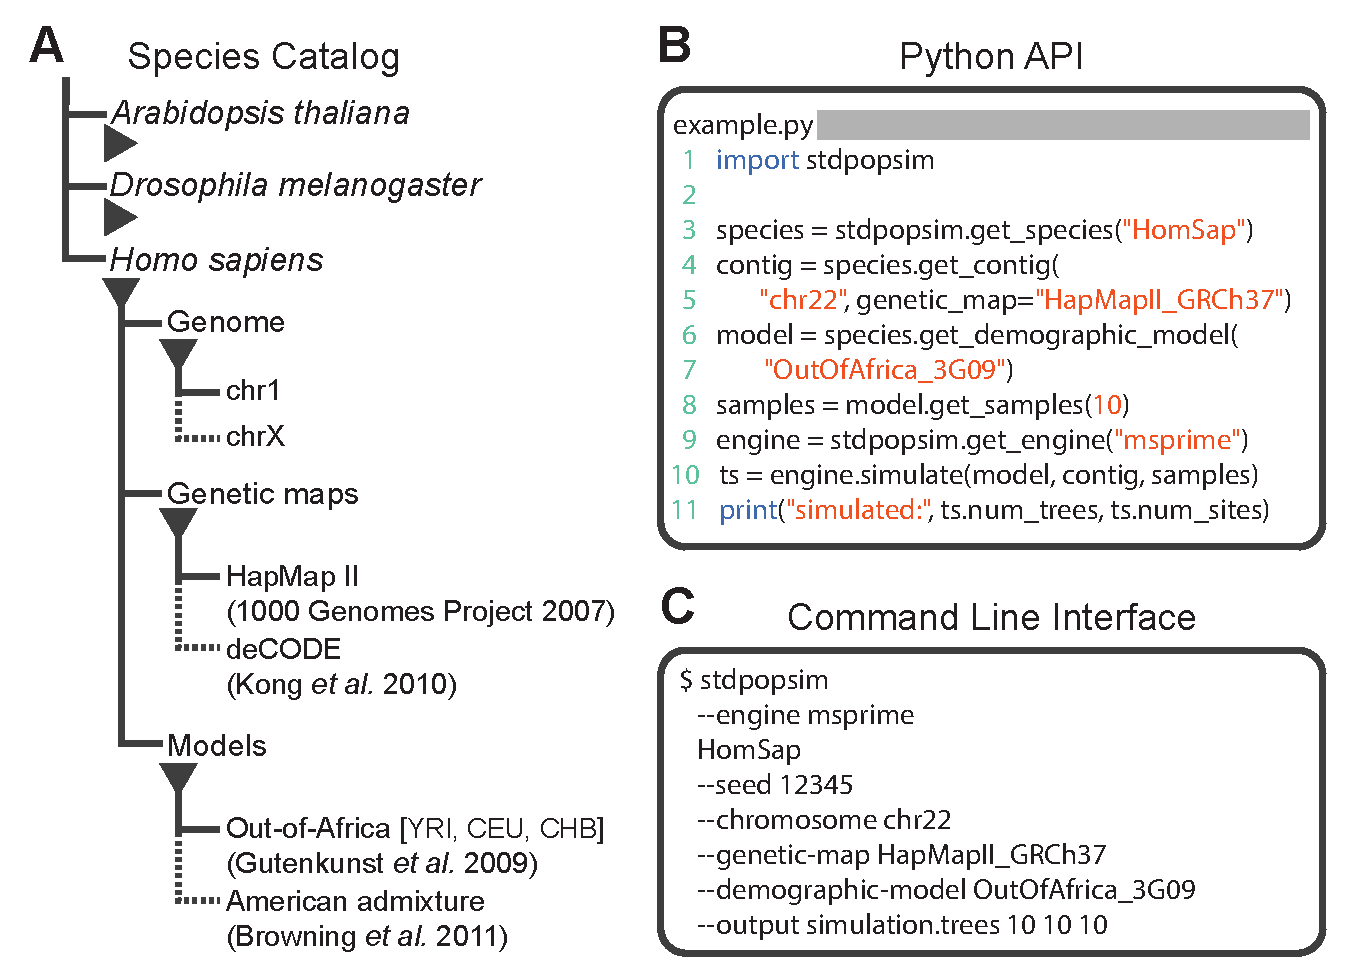
\includegraphics[width=0.5\linewidth]{display_items/Figure1.png}
\caption{\textbf{Structure of \stdpopsim}. \textbf{A.} The
hierarchical organization of the PopSim catalog contains all information
within individual species. Information within the species level is shown here
for \emph{Homo sapiens} only. We see that \emph{H. sapiens} is associated
with a default generation time and mutation rate, that it contains within
it a representation of the physical genome, genetic maps, and as shown a
subset of the demographic models currently implemented. \textbf{B.} Caching
and automated download of genetic maps. \textbf{C.} Example code to specify
and simulate models using \stdpopsim via the API (top) or
command-line interface (bottom). \textbf{D.} Simulation output from
\stdpopsim is generated as tree sequence files that can
be manipulated and analysed with \texttt{tskit}.}
\label{fig:cartoon}
\end{center}
\end{figure}

\section*{Results}
\paragraph{The \stdpopsim library}
The central contribution from PopSim currently is \stdpopsim, a community
maintained library of empirical genome data and population genetics simulation
models, providing easy access to realistic simulations. Figure \ref{fig:cartoon} shows a graphical
representation of the structure of \stdpopsim. The package centers
on a catalog of species (Fig. \ref{fig:cartoon}A), initially consisting of humans, \emph{Drosophila},
\emph{Arabidopsis}, \emph{E. coli}, and \emph{Pongo}. A species definition consists
of two key elements.  Firstly, the library defines
some basic information about its genome, with information about chromosome
lengths, average mutation rates and so on. We also provide access to detailed
empirical information such as recombination maps, which model empirically
observed heterogeneity along chromosomes. As such maps are often large and hard
to find, we provide a mechanism to automatically download (and cache locally) a
set of known maps (Fig. \ref{fig:cartoon}B). For example, in humans we support the HapMapII (\cite{international2007second}) and
Decode (\cite{kong2010fine}) genetic maps. The second key element of a species description
within \stdpopsim is a set of carefully curated population genetic model
descriptions from the literature, which are the basis for accurate simulations
of specific historical scenarios.

Given the genome data and simulation model descriptions defined within the
library, it is then straightforward to run accurate, standardized simulations
across a range of organisms. \stdpopsim has a Python API and a user-friendly
command line interface (Fig. \ref{fig:cartoon}C), allowing users with minimal experience direct access to
state-of-the-art simulations. Simulations are output in the “tree sequence”
format (\cite{kelleher2016efficient,kelleher2018efficient,kelleher2019inferring}), which
contains complete genealogical information about the simulated samples, is
extremely compact, and can be processed very efficiently using the tskit library
(\cite{kelleher2016efficient,kelleher2018efficient}; Fig. \ref{fig:cartoon}D). Currently,
\stdpopsim uses the  \texttt{msprime} coalescent simulator (\cite{kelleher2016efficient})
as the simulation engine. We plan to include other simulation
engines to support scenarios that cannot be modelled under the coalescent framework,
and have already implemented \texttt{SLiM} (\cite{haller2019slim}) as
an alternative back-end.

The \stdpopsim command line interface, by default, outputs citation information
for the models, genetic maps and simulation engines used in any particular run.
We hope that this will encourage users to appropriately acknowledge the
resources used in published work, and authors
of simulation models to contribute to our ongoing community-driven development process.

\subsection*{\texttt{stdpopsim} Catalog}
The current contents of the \texttt{stdpopsim} catalog are shown in Table X. At the time of
writing the PopSim Consortium has implemented previously published demographic models for
humans, \emph{Drosophila}, and \emph{Arabidopsis}. These include both
simpler, single population histories (e.g., in \emph{D. melanogaster} \cite{sheehan2016deep}),
and much more complex models which include population splitting, migration, and archaic
admixture (e.g., in humans \cite{ragsdale2019models}).

\begin{table}
\begin{footnotesize}
\begin{tabular}{lllS[table-format=3.1]S[table-format=3.1]S[table-format=2.1]}
\toprule
& Model ID & Citation & 
\multicolumn{1}{c}{ CPU(s) } 
&
\multicolumn{1}{c}{ RAM(MB) } 
&
\multicolumn{1}{c}{ File(MB) } 
\\
\midrule
\multicolumn{6}{l}{ HomSap (\emph{Homo sapiens}) } \\
&
Africa\_1T12& \cite{tennessen2012evolution} & 10.4& 193.3& 23.3\\
&
Zigzag\_1S14& \cite{schiffels2014inferring} & 3.4& 105.0& 7.9\\
&
AshkSub\_7G19& \cite{gladstein2019substructured} & 15.7& 215.3& 26.4\\
&
OutOfAfrica\_3G09& \cite{gutenkunst2009inferring} & 10.9& 181.3& 21.1\\
&
OutOfAfrica\_2T12& \cite{tennessen2012evolution} & 11.3& 198.0& 24.1\\
&
AncientEurasia\_9K19& \cite{kamm2019efficiently} & 69.4& 304.1& 41.2\\
&
AmericanAdmixture\_4B11& \cite{browning2018ancestry} & 11.1& 187.3& 22.3\\
&
PapuansOutOfAfrica\_10J19& \cite{jacobs2019multiple} & 234.7& 526.3& 77.8\\
&
OutOfAfricaArchaicAdmixture\_5R19& \cite{ragsdale2019models} & 9.6& 184.5& 21.7\\
\midrule
\multicolumn{6}{l}{ DroMel (\emph{Drosophila melanogaster}) } \\
&
OutOfAfrica\_2L06& \cite{li2006inferring} & 0.6& 68.7& 1.6\\
&
African3Epoch\_1S16& \cite{sheehan2016deep} & 0.5& 60.9& 0.2\\
\midrule
\multicolumn{6}{l}{ AraTha (\emph{Arabidopsis thaliana}) } \\
&
African2Epoch\_1H18& \cite{huber2018gene} & 434.1& 359.2& 50.7\\
&
African3Epoch\_1H18& \cite{huber2018gene} & 208.6& 400.6& 58.0\\
&
SouthMiddleAtlas\_1D17& \cite{durvasula2017african} & 159.6& 315.4& 43.1\\
\midrule
\multicolumn{6}{l}{ PonAbe (\emph{Pongo abelii}) } \\
&
TwoSpecies\_2L11& \cite{locke2011comparative} & 7.4& 170.5& 14.7\\
\bottomrule
\end{tabular}

\end{footnotesize}
\caption{\label{tab:catalog}
Details of the initial set of population models across four species.
\textbf{NOTES: Column names are ID, name (or description maybe?),
reference, CPU time, RAM}
}
\end{table}

At the time of writing, more models of human history have been implemented than for
any other organism. These models include: a simplified version of the \cite{tennessen2012evolution}
model with only the African population modeled (expansion from the ancestral
population and recent growth), the three population model of \cite{gutenkunst2009inferring}
which modeled the out-of-Africa bottleneck as well as the subsequent divergence of
the European and Asian populations, the \cite{tennessen2012evolution} two population variant of the
Gutenkunst model which did not include Asian populations, but more explicitly modeled
recent recent human population growth, the \cite{browning2018ancestry} admixture model
for American populations that models ancestral African, European, and Asian population
components, and the three population out-of-Africa model that includes archaic admixture
from \cite{ragsdale2019models}. Together these models
contain features found in real data (e.g. bottlenecks, population growth,
admixture) which are pertinent in the context of method development.

For non-human genomes we have have implemented two demographic histories for
\emph{Drosophila melanogaster} and one each from \emph{A. thaliana} and \emph{E. coli}.
For \emph{D. melanogaster} we have implemented the three epoch model estimated from
an African sample from \cite{sheehan2016deep} as well as the out-of-Africa divergence
and associated bottleneck model of \cite{li2006inferring} which jointly models African
and European populations. For For \emph{Arabidopsis thaliana}, we implemented the
model from in \cite{durvasula2017african} inferred using \MSMC. This model includes
a continuous change in population size over time, rather than pre-specified epochs of different
population sizes.


\subsection*{Use case: comparing methods of demographic inference}
As an example of the utility of \stdpopsim we demonstrate how popular
methods can be simply and fairly compared in the setting of demographic
inference using our resource. Although we present comparison of results from several
competing methods, our aim at this stage is not to provide an exhaustive
evaluation of these methods. Our hope is instead that future work built upon this resource
will enable more detailed exploration of the strengths and weaknesses of the numerous
inference methods that are available to the population genetics community.

We start by comparing popular methods for estimating
population size histories ($N(t)$) of single populations and subsequently
show simple examples of multi-population inference.
To evaluate and compare the performance of inference methods we developed
\texttt{snakemake} (\cite{koster2012snakemake}) workflows that allow reproducibility
in comparing inference methods which are available from \url{https://github.com/popgensims/analysis}
. The workflows allow efficient computing in multicore environments or on
cluster environments.

For single-population population size histories, we compared \MSMC, \smcpp, and
\stairwayplot (\cite{schiffels2014inferring,terhorst2017robust,liu2015exploring})
 on simulated genomes sampled from a single population,
in a number of the \stdpopsim models described above. The pipeline was generalized to
run $R$ replicates with $C$ chromosomes for $N$ samples, for a total of $R \times C$
simulations for each demographic model. After simulation, the pipeline prepares
input files for each of the respective inference methods by grouping all
chromosomes, for each sample, into a single file. This step results in an
input file for each simulation replicates $R$, pertaining to each of the
respective inference methods and derived from the same simulated tree sequences.
Each of the inference programs are then run in parallel, followed by plotting of
$N_e$ estimates from each program.

\begin{figure}
\begin{center}
\includegraphics[width=0.8\linewidth]{display_items/homo_sapiens_mask_Ragsdale.png}
\caption{\textbf{Comparing estimates of $N(t)$ in humans}. Here we show estimates of population
size over time ($N(t)$) inferred using 4 different methods, \smcpp, \texttt{stairwayplot},
\MSMC with $n=2$ and $n=8$. Data were generated by simulating
replicate human genomes under the \cite{ragsdale2019models} model and using the genetic map
inferred in \cite{international2007second}. From top to bottom we show estimates for each
of the three populations in the model YRI, CEU, and CHB. In shades of blue we show the estimated
$N(t)$ trajectories for each replicate. In black we show the true population size history as inferred
for the rate of coalescence in the demographic model.}
\label{fig:n_t_ragsdale}
\end{center}
\end{figure}


In Figure \ref{fig:n_t_ragsdale} we present results from our $N(t)$ analysis pipeline
run on whole genome simulations under the \cite{ragsdale2019models} model using the
human genetic map estimated from \cite{international2007second}. On rows
we show inferred $N(t)$ for the three extant populations in the model.
On columns we show comparisons among the methods (note that we compare two differing
sample sizes for \MSMC). The solid black lines represent the true effective population
size as inferred from the inverse coalescent rate defined by the model.
Blue lines represent estimates from each of three replicate whole genome simulations.
While there is variation among methods and individual population estimates,
generally spoken the methods are accurate for this model of human history.

\stdpopsim allows us to readily compare these estimates to those drawn from a different
model of human history. In Figure \ref{fig:n_t_gutenkunst} we show estimates of
$N(t)$ from simulations using the same physical and genetic maps, but a different demographic
history-- that inferred by \cite{gutenkunst2009inferring}. Again we see that each
of the methods is capturing relevant parts of the population history, although the
degree of noise at any given time interval varies. In comparing inferences between the
models it is interesting to note that $N(t)$ estimates for the CHB and CEU
simulated populations are generally better across methods than estimates from the YRI
sample.


\begin{figure}
\begin{center}
\includegraphics[width=0.8\linewidth]{display_items/d_mel_Sheehan_mask2.png}
\caption{\textbf{Comparing estimates of $N(t)$ in \emph{Drosophila}}. Population
size over time ($N(t)$) estimated from an African population sample. Data were generated by simulating
replicate \emph{D.melanogaster} genomes under the three-epoch \cite{sheehan2016deep} model
with the genetic map inferred in \cite{comeron2012many}. In shades of blue we show the estimated
$N(t)$ trajectories for each replicate. In black we show the true population size history as inferred
for the rate of coalescence in the demographic model.}
\label{fig:n_t_sheehan}
\end{center}
\end{figure}

As most population genetic methods development has been focused on human-scale
data, it is of consequence to ask how such methods might perform in non-human
genomes. Figure \ref{fig:n_t_sheehan} shows parameter estimates from a demographic
model estimated from an African sample of \emph{Drosophila melanogaster} (\cite{sheehan2016deep}).
As with humans, we use \stdpopsim to simulate replicate \emph{Drosophila} genomes under
an empirically derived genetic map, and then try to infer back the parameters of model.
Accuracy is mixed among methods in this setting, and generally worse than what we
observe under simulations of the human genome.

\adk{do we want to include Arabidopsis results too?}


\begin{figure}
\begin{center}
\includegraphics[width=0.7\linewidth]{display_items/homo_sapiens_two_popn_comp.png}
\caption{\textbf{A comparison two-population parameter estimates in humans}. Here we show estimates of $N(t)$ inferred using \dadi, \texttt{fastsimcoal2}, or \smcpp.
A) Data were generated by simulating
replicate human genomes under the \cite{gutenkunst2009inferring} model and using the genetic map
inferred in \cite{international2007second}. B) For \dadi and \texttt{fastsimcoal2} we show inferred
parameters out of the depicted IM model, inferring population sizes, migration rates, and a split
time between CEU and YRI samples. C) Population size estimates for each population (rows)
from \dadi, \texttt{fastsimcoal2}, and \smcpp (columns). In shades of blue we show the estimated
$N(t)$ trajectories for each replicate. In black we show the true population size history as inferred
for the rate of coalescence in the demographic model. The population split date, $T_{div}$, is shown as
an inset panel, with a common X-axis to the background figure.}
\label{fig:IM_popn_human}
\end{center}
\end{figure}

\paragraph*{Multi Population demographic models}
As \texttt{stdpopsim} implements multi-population demographic models, we also
explored parameter estimation of population divergence parameters. In particular
we performed simulations under multi-population models for humans and Drosophila
and inferred simulated parameters using \dadi, \fastsimcoal, and \smcpp.
For simplicity, we conducted inference in \dadi and \fastsimcoal using an IM model
with constant population sizes and bi-directional migration. For human
models with more than two-populations, e.g. \cite{gutenkunst2009inferring},
this means that we are inferring parameters from a model which itself does
not match the model from which the data were generated (Figure
\ref{fig:IM_popn_human}A and B), however this is common practice in the field
when applying IM-type models.

In Figure \ref{fig:IM_popn_human}C we show estimates of population sizes and divergence
time from each of the methods for samples simulated for the African and European populations
under the \cite{gutenkunst2009inferring} model. Each of the methods compared has stronger
and weaker points to their accuracy across parameters. For instance the simple, IM-style
analyses we have performed do not capture recent population size change in CEU, however
they do a good job of estimating the quite simple YRI population size history.

Again we can compare between genomes and look at the performance of these methods in
the context of a two population model from \emph{Drosophila melanogaster}. Figure
\ref{fig:two_popn_fly} shows parameter estimates from simulations drawn from
the model from \cite{li2006inferring} which includes
an ancestral population in Africa, then a population expansion with a population
split and bottleneck into a European population. These simulations are generated
using the recombination map of \cite{comeron2012many}. Here methods differ dramatically
in the estimates, with \smcpp yielding quite noisy estimates of population size
towards the more ancient past and all methods failing to capture the very brief
population bottleneck in Europe, although the IM-model of course only allows for
two epochs in the population size history.

Again the goal of these analyses are not to perform thorough benchmarking of
the methods at hand under a wide range of simulations, but instead to show how
the tools that we have built could be used to do so.

\section*{Discussion}
Here we have described what we view as the first product from the PopSim Consortium:
the \stdpopsim library. We have founded the Consortium with a number of specific aims
in mind: standardization of simulation within the computational genetics community,
increasing reproducibility of simulation based results, community-based development and
decision making in guiding best practices in population genetics, and eventual benchmarking
of inferential methods.

The \stdpopsim library is the first piece of this effort, in that it allows for rigorous
standardization of complex population genetic simulations. Population genetics, as a field,
has yet to coalesce around a set of gold-standards for the crucial task of simulation.
Moreover individual research groups are often in the position of having to independently
reimplement complex, previously published models. \stdpopsim offers solutions to both of
these issues by creating a quality controlled, easy-to-use, gateway to models and organisms
that are central to modern research in genetics.

We have built \stdpopsim, and the PopSim Consortium, to be an open, community-developed
project, meaning that it has excellent potential for future growth.
Thus far we have implemented genome representations and genetic maps for the three most
common study systems in computational genetics: humans, \emph{Drosophila}, and \emph{Arabidopsis}.
The standard operating procedures that we have outlined in our detailed documentation
means that new researchers, who are interested in adding their favorite organism/genome
are free to with very few barriers to entry. Further new demographic models can be added
to each of the organisms in the catalog through similarly well documented steps.
A long-term goal then is that through a mechanism such as \stdpopsim, the community
can determine (in an open way) what is the correct implementation for a given model,
and in turn, what are the models that the community is most interested in.

We have shown in the results above how \stdpopsim can be used for direct comparisons
of inferential methods on a common set of simulations. While we have not made a concerted
effort at benchmarking methods yet, we believe that this would be an important effort for
the PopSim Consortium and population genetics more broadly. The analysis workflows that
we have released as part of \stdpopsim should provide a cookbook for the community to
dive in to more rigorous benchmarking than we have done thus far.

\adk{should we mention benchmarking of tree sequence inference here? what else?}


\section*{Methods}
\subsection*{Generating the PopSim resource}

\subsection*{Model QC procedures}
Each demographic model was implemented independently by two people working from
the relevant primary sources. Disagreements between complete implementations
were resolved between the implementers in consultation with the authors of the
source papers when necessary. A comparison of the two implementations is then
added as a unit test.Technical details of the QC process can be found in the
GitHub repository in the developer documentation.

\subsection*{Workflow for analysis of simulated data}
Snakemake pipeline for 1 pop models
Snakemake pipeline for 2 pop models

 In general, used default
settings and did not attempt to optimize \dadi or \fastsimcoal runs Used Snakemake to
manage pipeline for two population analysis Results from two population pipeline
demonstrate that the different methods tested were generally able to recover the
simulated parameters


% \subsection*{Extra text}
% [This section describes the stdpopsim Python library. What it’s for, how it’s used and what it can do]
% [First para: running accurate simulations is hard]
% Running realistic population genetic simulations is a complex task today. It is
% straightforward to run simple simulations of population models such as the
% coalescent or Wright-Fisher using (e.g.) msprime or SLiM, but the process of
% instantiating these models to accurately reflect the properties of natural
% populations that are important for a particular study is fraught with
% difficulties. There are typically three important inputs that must be decided:
% the demographic model, recombination and mutation rates. Demographic models for
% a particular species are typically chosen by examining the literature for
% published model specifications, which can consist of dozens of parameters. These
% parameters must be transcribed from the original publication and translated into
% the input format required for the simulator in question. This is a difficult and
% error prone task, and mistakes are common. Recombination and mutation rates are
% simpler to describe and often a single genome-wide estimate is appropriate.
% However, such estimates are updated frequently and there is wide variation in
% the values used for the simulations of the same species. When more fine-grained
% simulations of the local chromosome structure is required, empirical
% recombination and mutation rate maps are used. However, there is no standard
% format for such maps, and finding the maps can be challenging.



\bibliographystyle{plainnat}
\bibliography{PopSim.bib}

\pagebreak
\beginsupplement
\section*{Supplemental Figures}
\begin{figure}
\begin{center}
\includegraphics[width=0.8\linewidth]{display_items/homo_sapiens_mask_Gutenkunst.png}
\caption{\textbf{Comparing estimates of $N(t)$ in humans}. Here we show estimates of population
size over time ($N(t)$) inferred using 4 different methods, \smcpp, \stairwayplot,
\MSMC with $n=2$ and $n=8$. Data were generated by simulating
replicate human genomes under the \cite{gutenkunst2009inferring} model and using the genetic map
inferred in \cite{international2007second}. From top to bottom we show estimates for each
of the three populations in the model YRI, CEU, and CHB. In shades of blue we show the estimated
$N(t)$ trajectories for each replicate. In black we show the true population size history as inferred
for the rate of coalescence in the demographic model.}
\label{fig:n_t_gutenkunst}
\end{center}
\end{figure}

\begin{figure}
\begin{center}
\includegraphics[width=0.8\linewidth]{display_items/d_mel_two_popn_comp.png}
\caption{\textbf{A comparison two-population parameter estimates in Drosophila}. Here we show estimates of $N(t)$ inferred using \dadi, \texttt{fastsimcoal2}, or \smcpp.
Data were generated by simulating
replicate human genomes under the \cite{li2006inferring} model and using the genetic map
inferred in \cite{comeron2012many}. See legend of Figure \ref{fig:IM_popn_human} for details.
In shades of blue we show the estimated
$N(t)$ trajectories for each replicate. In black we show the true population size history as inferred
for the rate of coalescence in the demographic model.}
\label{fig:two_popn_fly}
\end{center}
\end{figure}

\stopsupplement

\end{document}
